
\subsection{Angles}

\textit{Demonstrate knowledge of \textbf{complementary}, \textbf{supplementary}, and \textbf{vertical} angles.}

\vspace{.25cm}

\say{In Euclidean geometry, an angle is the figure formed by two rays, called the sides of the angle, sharing a common endpoint, called the vertex of the angle.}\href{https://en.wikipedia.org/wiki/Angle}{Wikipedia}



\paragraph*{complementary angles}

The sum of two \textbf{complementary} angles is $90^\circ$.

\begin{figure}[h!]
    \centering
    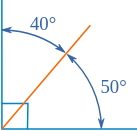
\includegraphics[width=2cm]{./public/images/complementary}
    \caption[short]{complementary angles}
\end{figure}

\say{The adjective complementary is from the Latin complementum, associated with the verb complere, "to fill up". An acute angle is "filled up" by its complement to form a right angle.}

\paragraph{supplementary angles}add up to $ 180^\circ$.

\begin{figure}[h!]
    \centering
    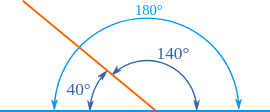
\includegraphics[width=4cm]{./public/images/supplementary}
    \caption[short]{supplementary angles}
\end{figure}

\paragraph*{vertical angles}

\href{https://en.wikipedia.org/wiki/Angle#Vertical_and_adjacent_angle_pairs}{vertical angles}are formed by two intersecting lines.